\appendix

\chapter{Bayesian Regression Posterior Updates}

\section{Normal Prior with Known Noise}{\label{a:bn}

The following development of the posterior updates for the BN model is summarized from chapter 2.1 in \cite{rasmussen_2006} but with the slight modification of allowing a non-zero mean prior. 

Start with the linear regression model $y=X\beta + \varepsilon$. In this setting it is assumed that this models a deterministic process with mean $X\beta$ and variance $\sigma^2$. Assuming that the targets $y_i$ are independent the likelihood function over the training data is given by
%8-11
\begin{equation}
    \begin{split}
        p(y|X,\beta) &= \sum^n_{i=1} \frac{1}{\sqrt{2\pi}\sigma}\exp\Bigg(-\frac{(y_i - x_i^T\beta)^2}{2\sigma^2}\Bigg)\\
        &=\frac{1}{(2\pi\sigma^2)^\frac{n}{2}}\exp\bigg(\frac{1}{2\sigma^2}|y - X\beta|^2\bigg)\\
        &= N(X\beta, \sigma^2\bm{I})
    \end{split}
\end{equation}

Consider the bayesian setting where the coefficients $\beta$ are random variables but the noise variance $\sigma^2$ is known. One choice of prior distribution is the normal distribution $N(\mu, \sigma)$ as this is a conjugate prior in this case.

Using bayes rule it can then be shown that

\begin{equation}
    \label{eq:post_proof_bn}
    \begin{split}
        p(\beta|X,y) &\propto \exp\bigg[-\frac{1}{2\sigma^2}\big(y-X\beta\big)^T\big(y-X\beta\big)\exp\bigg(-\frac{1}{2}\beta^T\Sigma^{-1}\beta\bigg)\bigg] \\
        &\propto \exp\bigg[-\frac{1}{2}\Big(\beta-\tilde{\beta}\Big)^T\Big(\frac{1}{\sigma^2}X^TX + \Sigma^{-1}\Big)\Big(\beta - \tilde{\beta}\Big)\bigg]
    \end{split}
\end{equation}

where $\tilde{\beta} = \sigma^{-2}(\sigma^{-2}X^TX + \Lambda^{-1})^{-1}(\Lambda\mu + X^Ty)$ and $\Lambda = \Sigma^{-1}$. This form matches the quadratic form of the normal distribution meaning the posterior coefficients are distributed

\begin{equation}
    p(\beta |X,y) \sim N\bigg(\sigma^{-2}\big(\sigma^{-2}X^TX + \Lambda\big)^{-1}\big(\Lambda\mu + X^Ty\big), \quad \sigma^{-2}X^TX + \Lambda\bigg).
\end{equation}

Here it can be seen that the normal distribution is in fact a conjugate prior as the posterior of $\beta$ is also normal. The posterior update can finally be written as seen in equation \ref{eq:known_noise_posterior_update}.

\section{Normal Inverse Gamma Prior}{\label{a:bnig}

For the bayesian setting where both $\beta$ and $\sigma^2$ are unknown the result is summarized from section 4.4.1 in \cite{fahrmeir_2013}. In this case one keeps the normal prior over the $\beta$ coefficients and assigns $\sigma$ the prior

\begin{equation}
    \sigma^2 \sim \text{InvGamma}(a,b) = \frac{b^a}{\Gamma(a)}\frac{1}{(\sigma^2)^{a+1}}\exp\bigg(-\frac{b}{\sigma^2}\bigg).
\end{equation}

Under the assumption that the noise term is homoscedastic the joint prior can then be written as 

\begin{equation}
    \begin{split}
        p(\beta, \sigma^2) &= p(\beta|\sigma^2)p(\sigma^2)  \\
        &=\frac{1}{(2\pi\sigma^2)^\frac{p}{2}|\Sigma|^\frac{1}{2}}\exp\Big(-\frac{1}{2\sigma^2}\big(\beta-\mu\big)^T\Lambda\big(\beta-\mu\big)\Big)\cdot\\
        & \qquad \frac{b^a}{\Gamma(a)}\frac{1}{(\sigma^2)^{a+1}}\exp\Big(-\frac{b}{\sigma^2}\Big) \\
        &\propto \frac{1}{(\sigma^2)^{\frac{p}{2}+a+1}}\exp\Big(-\frac{1}{2\sigma^2}\big(\beta-\mu\big)^T\Lambda\big(\beta-\mu\big) - \frac{b}{\sigma^2}\Big)
    \end{split}
\end{equation}

Bayes rule then states that 

$$
p({\beta},\sigma^{2}|y ,X) \propto p(y|X,\beta,\sigma^{2})p(\beta|\sigma^{2})p(\sigma^{2}).
$$

which gives

\begin{equation}
    \begin{split}
        p(\beta, \sigma^2&|y,X) \propto \\
        &(\sigma ^2)^{-\frac {n}{2}}\exp\Big[-\frac{1}{2\sigma^2}(y-X \beta)^T(y -X\beta)\Big]\\
        &(\sigma^2)^{-\frac{k}{2}}\exp\Big[-\frac {1}{2{\sigma }^2}(\beta-\mu_0)^{T}{\Lambda }_0(\beta-\mu_0)\Big]\\
        &(\sigma^2)^{-(a_0+1)}\exp\Big[-\frac{b_0}{\sigma^2}\Big].
    \end{split}
\end{equation}

In section 4.5.2 in \cite{fahrmeir_2013} a proof is given that shows

\begin{equation}
    \begin{split}
        (y-X\beta)^T&(y-X\beta) + (\beta-\mu_0)^T\Lambda_0(\beta-\mu_0) \\
        = &y^Ty + (\beta - \mu_n)^T\Lambda(\beta-\mu_n) - \mu_n^T\Lambda\mu_n + \mu_0^T\Lambda\mu_0
    \end{split}
\end{equation}

where $_0$ denotes the prior and 

\begin{align*}
    \Lambda_{n} & = X^TX + \Lambda_{0} \\
    \mu_{n}     & = \Lambda_{n}^{-1}(\Lambda_{0}\mu_{0} + X^Ty)
\end{align*}

which one recognizes as the posterior updates for the BN model without the noise term. This leaves the expression

\begin{equation}
    \begin{split}
        p(\beta, \sigma^2&|y,X) \propto \\
        & \exp\bigg[-\frac{1}{2\sigma^2}\Big(\beta-\mu_n\Big)^T\Lambda_n\Big(\beta-\mu_n\Big)\bigg] \\
        &\frac{1}{(\sigma^2)^{a_0+\frac{n}{2}+1}}\exp\bigg[-\frac{b_0+y^Ty  - \mu_n^T\Lambda\mu_n + \mu_0^T\Lambda\mu_0}{\sigma^2}\bigg]
    \end{split}
\end{equation}

which shows that the normal inverse gamma prior is a conjugate prior with the posterior update shown in equation \ref{eq:unknown_noise_posterior_update}.

\chapter{Linear Model Experiments}

\vspace{-1cm}

\section{2 State Propagation}\label{a:2_state_exp}

\begin{figure}[H]
    \centering
    \begin{tikzpicture}[shorten <=2pt,shorten >=2pt,->,>=stealth',auto,node distance=3cm,
        thick,main node/.style={circle,draw,font=\sffamily\Large\bfseries}]

        \node[main node] (1) {1};
        \node[main node] (2) [right of=1] {2};

        \path[every node/.style={font=\sffamily\small}]
            (1) edge node {r=0} coordinate [pos=0.5] (middle)(2);
    \end{tikzpicture}
    \caption{\textbf{2 State Toy Environment}}
    \label{fig:app_2state}
\end{figure}

For the 2 state propagation experiments a regression model $\mathcal{M}$ with the form $y = X\beta + \varepsilon$ where $\beta = [\begin{array}{cc}\beta_1  & \beta_2\end{array}]$ was used. Since state 2 has a known posterior $\mathcal{M}$ only trains on state 1. This means $x$ is always $[\begin{array}{cc}1  & 1\end{array}]$. The pseudocode for the two target methods follows. 

\begin{algorithm}[H]
    \caption{Sample Target Variance Propagation}
    Initialize a model of choice $\mathcal{M}$\\
    \For{iteration = 1, 1000}{
        $y = \text{sample from} \; N(1,\sigma^2)$\\
        Update $\mathcal{M}$ priors given input $(x, y)$
    }
\end{algorithm}

\begin{algorithm}[H]
    \caption{Mean Target Variance Propagation}
    Initialize a model of choice $\mathcal{M}$\\
    \For{iteration = 1, 1000}{
        $y = 1$ \\
        Update $\mathcal{M}$ priors given input $(x, y)$
    }
\end{algorithm}

\section{N State Propagation}\label{a:n_state_exp}

The N state propagation experiments were only running using BNIG models. One model was made per unknown state and each model was trained on one sample from the next state every iteration. This is summarized in the following pseudocode:

\begin{algorithm}[H]
    \caption{Multiple State Variance Propagation}
    $s = \text{number of states}$ \\
    $\mathcal{M}$ = array of $s-1$ of BNIG models\\
    \For{iteration = 1, T}{
        \For{i = 1, $s-2$}{
            Sample $\beta, \sigma$ from $\mathcal{M}$[i+1] \\
            Sample $\varepsilon \sim N(0, \sigma^2)$ \\
            $y = x^T\beta + \varepsilon$\\
            Update $\mathcal{M}[i]$ priors given input $(x, y)$
        }
        $y = \text{sample from} \; N(1,\sigma^2)$\\
        Update $\mathcal{M}[s-1]$ given input $(x, y)$
    }
\end{algorithm}

The 3 state experiments were run for 10000 iterations while the 6 state experiments were run for 1000 iterations.

Instructions on how to run the code for all the propagation experiments can be found in the readme file that comes with the provided code.

\section{Linear Corridor Experiment}{\label{a:lin_corridor}}

The code ReadMe contains instructions on how to run the linear corridor experiment presented in chapter \ref{ch:linear}. The hyperparameters used to create the linear corridor experiment figure \ref{fig:linear_corridor}   are given below. A short description per hyperparameter is also provided

\subsection{Environment Details}

The environment consists of N states and lasts N timesteps. A right action leads to 0 reward unless it reaches the final right state in which case it returns a reward of 1. Every left action returns a reward of $\frac{1}{10N}$. The left action is encoded by 0 and the right by 1. The output from the environment is an array of two values, one for the current timestep and one for the current state.

\subsection{Hyperparameters}

\subsubsection{$\varepsilon$-Greedy}

The $\varepsilon$-greedy method has few hyperparameters. The learning rate is the learning rate used for the stochastic gradient descent over the regression parameters and is often denoted by $\alpha$ in RL literature. The $\varepsilon$ term is the probability of performing a random action. This is decayed during training from some initial $\varepsilon$ to a final $\varepsilon$ over a set number of episodes.

\begin{table}[H]
    \centering
    \begin{tabular}{@{}lr@{}}
        \toprule
        Hyperparameter                     & Value \\ \midrule
        Learning Rate                      & 0.01  \\
        Initial $\varepsilon$              & 1     \\
        Final $\varepsilon$                & 0.001 \\
        Num. episodes for decay            & 200   \\ \bottomrule
    \end{tabular}
    \caption{Linear Corridor $\varepsilon$-Greedy hyperparameters}
\end{table}

\subsubsection{BN}

The hyperparameters for the BN model consist of the priors, the "known" noise variance and the decay rate for the exponential forgetting. The $\beta$ prior mean is se equal for all coefficients, with a value denoted $\mu$. The prior $\beta$ covariance is set have the value $\sigma^2_\beta$ along the diagonal and zero otherwise. The noise term $\sigma^2_\varepsilon$ is assumed known but treated as a hyperparameter. Finally the decay rate defines the discount factor used for the exponential forgetting of previous data. The terms used to update the posterior are multiplied by this factor terms as in formula \ref{eq:exponential_forgetting}.

\begin{table}[H]
    \centering
    \begin{tabular}{@{}lr@{}}
        \toprule
        Hyperparameter               & Value \\ \midrule
        Prior $\mu$                  & 0     \\
        Prior $\sigma_\beta^2$       & 0.001 \\
        $\sigma^2_\varepsilon$       & 1e-12 \\
        Decay Rate                   & 0.999 \\ \bottomrule
        \end{tabular}
        \caption{Linear Corridor BN hyperparameters}

\end{table}

\subsubsection{BNIG}

The BNIG hyperparameters are the same as the BN model apart from the known noise term which is replaced by the inverse gamma prior parameters. These two parameters are $a$ and $b$.

\begin{table}[H]
    \centering
    \begin{tabular}{@{}lr@{}}
        \toprule
        Hyperparameter               & Value \\ \midrule
        Prior $\mu$                  & 0     \\
        Prior $\sigma_\beta^2$       & 1 \\
        Prior $a$                    & 1 \\
        Prior $b$                    & 0.01\\
        Decay Rate                   & 0.999 \\ \bottomrule
        \end{tabular}
        \caption{Linear Corridor BNIG hyperparameters}
\end{table}


\chapter{Neural Network Experiments}

\section{Environment Hyperparameters}

The prior parameters were set to the same value across all environments


\begin{table}[H]
    \centering
    \begin{tabular}{@{}lr@{}}
        \toprule
        Hyperparameter               & Value \\ \midrule
        Prior $\mu$                  & 0 \\
        Prior $\sigma_\beta^2$       & 1 \\
        Prior $a$                    & 1 \\
        Prior $b$                    & 0.01\\ \bottomrule
    \end{tabular}
    \caption{BNIG DQN Priors}
\end{table}

\subsection{Corridor}

The corridor neural network contained one hidden layer with 20 neurons with ReLu activation functions.

\begin{table}[H]
    \centering
    \begin{tabular}{@{}lr@{}}
        \toprule
        Hyperparameter               & Value \\ \midrule
        Learning rate                & 0.001 \\
        Discount factor $\gamma$     & 0.99  \\
        $N$-step                     & 3-step \\
        Train DQN Interval           & 10 steps \\
        Target Sync Interval         & 10 steps \\
        Batch Size                   & 128 \\
        Max Replay Capacity          & 100000 \\ 
        Initial $\varepsilon$        & 1 \\
        Final $\varepsilon$          & 0 \\
        $\varepsilon$ Decay Steps    & 250000 \\ \bottomrule
    \end{tabular}
    \quad
    \begin{tabular}{@{}lr@{}}
        \toprule
        Hyperparameter               & Value \\ \midrule
        Learning rate                & 0.001 \\
        Discount factor $\gamma$     & 0.99  \\
        $N$-step                     & 3-step \\
        Train DQN Interval           & 10 \\
        Target Sync Interval         & 10\\
        Batch Size                   & 128 \\
        Max Replay Capacity          & 100000 \\
        Exponential Forgetting Rate  & 0.999 \\ \bottomrule
    \end{tabular}
    \caption{Nerual network corridor hyperparameters: \textbf{Left}: DQN Priors. \textbf{right}:BNIG DQN Priors}
\end{table}

\subsection{Cartpole and Acrobot}

The same neural network and hyperparameters were used in cartpole and acrobot. The neural network consisted of two hidden layers with 512 neurons each and ReLu activation functions.

\begin{table}[H]
    \centering
    \begin{tabular}{@{}lr@{}}
        \toprule
        Hyperparameter               & Value \\ \midrule
        Learning rate                & 0.001 \\
        Discount factor $\gamma$     & 0.99  \\
        $N$-step                     & 10-step \\
        Train DQN Interval           & 4 steps \\
        Target Sync Interval         & 100 steps \\
        Batch Size                   & 128 \\
        Max Replay Capacity          & 100000 \\ 
        Constant $\varepsilon$       & 0.01 \\ \bottomrule
    \end{tabular}
    \quad
    \begin{tabular}{@{}lr@{}}
        \toprule
        Hyperparameter               & Value \\ \midrule
        Learning rate                & 0.001 \\
        Discount factor $\gamma$     & 0.99  \\
        $N$-step                     & 10-step \\
        Train DQN Interval           & 4 \\
        Target Sync Interval         & 100 \\
        Batch summarized             & 128 \\
        Max Replay Capacity          & 100000 \\
        Exponential Forgetting Rate  & 1-1e-5 \\ \bottomrule
    \end{tabular}
    \caption{Acrobot and Cartpole hyperparameters: \textbf{Left}: DQN Priors. \textbf{right}:BNIG DQN Priors}
\end{table}

\subsection{Pong}

The atari setup followed the setup used in \cite{mnih_2015}. This consists of resizing the input image to 84x84 and scaling the pixel values between 0 and 1. Finally the 4 previous frames are stacked before being sent into the network. The network consists of three 2D convolutional layers(details in table \ref{tb:conv_net}) followed by a flattening operation that is sent into a final hidden layer with 512 neurons with ReLu activation functions.

\begin{table}[H]
    \caption{Convolutional Layers}
    \label{tb:conv_net}
    \centering
    \begin{tabular}{@{}cccc@{}}
        \toprule
        Layer & Filters & Size & Stride \\ \midrule
        1 & 32 & 8x8 & 4 \\
        2 & 64 & 4x4 & 2 \\
        3 & 64 & 3x3 & 1 \\ \bottomrule
    \end{tabular}
\end{table}

\begin{table}[H]
    \centering
    \begin{tabular}{@{}lr@{}}
        \toprule
        Hyperparameter               & Value \\ \midrule
        Learning rate                & 0.001 \\
        Discount factor $\gamma$     & 0.99  \\
        $N$-step                     & 5-step \\
        Train DQN Interval           & 4 steps \\
        Target Sync Interval         & 8000 steps \\
        Batch Size                   & 32 \\
        Max Replay Capacity          & 1000000 \\ 
        Constant $\varepsilon$       & 0.01 \\ 
        Initial $\varepsilon$        & 1 \\
        Final $\varepsilon$          & 0.01 \\
        $\varepsilon$ Decay Steps    & 250000 \\ \bottomrule
    \end{tabular}
    \quad
    \begin{tabular}{@{}lr@{}}
        \toprule
        Hyperparameter               & Value \\ \midrule
        Learning rate                & 0.00025 \\
        Discount factor $\gamma$     & 0.99  \\
        $N$-step                     & 5-step \\
        Train DQN Interval           & 4 \\
        Target Sync Interval         & 000 \\
        Batch summarized             & 32 \\
        Max Replay Capacity          & 1000000 \\
        Exponential Forgetting Rate  & 1-1e-5 \\ \bottomrule
    \end{tabular}
    \caption{Atari hyperparameters: \textbf{Left}: DQN Priors. \textbf{right}:BNIG DQN Priors}
\end{table}

\clearpage

\section{Per Seed Plots}


\begin{figure}[H]
    \centering
    \subfloat[DQN]{
        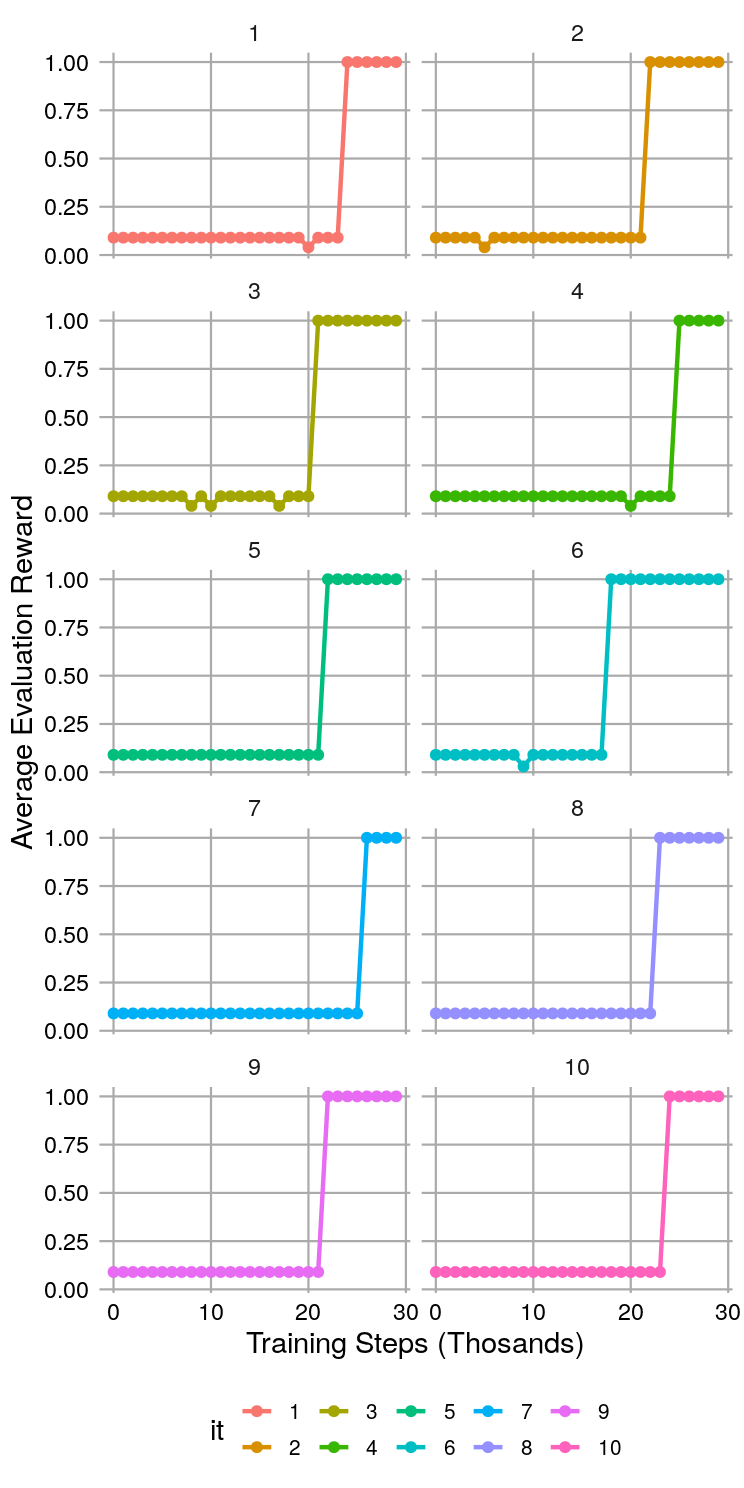
\includegraphics[scale=0.5]{PerDQNCorridor.png}
    }
    \subfloat[BNIG DQN]{
        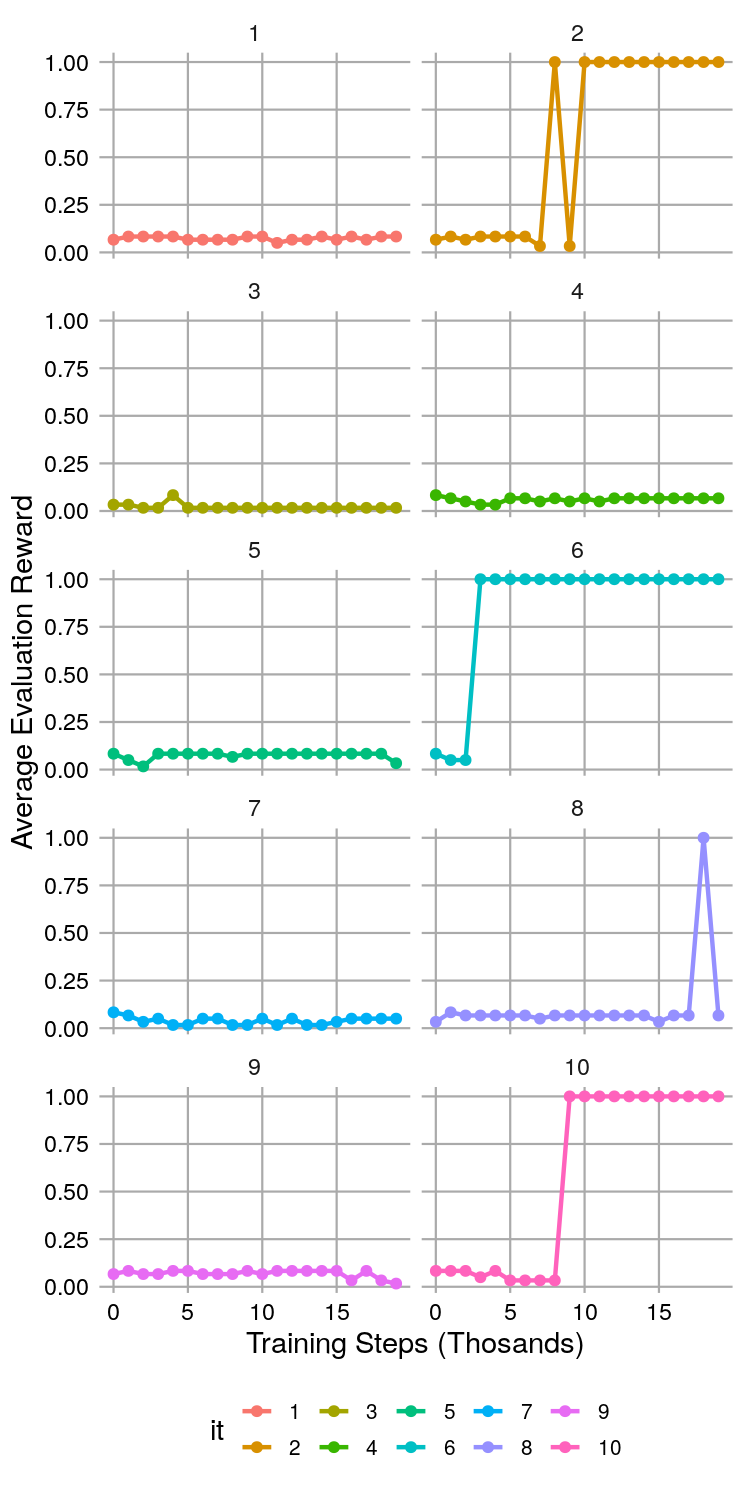
\includegraphics[scale=0.5]{PerBDQNCorridor.png}
    }
    \caption{\textbf{Per Seed DQN and BNIG DQN Performance on Corridor}:  Each color represents a new attempt. The DQN consistently finds a successful policy. The BNIG DQN never finds one.}
    \label{fig:nn_per_corridor}
\end{figure}


\begin{figure}[H]
    \centering
    \subfloat[DQN]{
        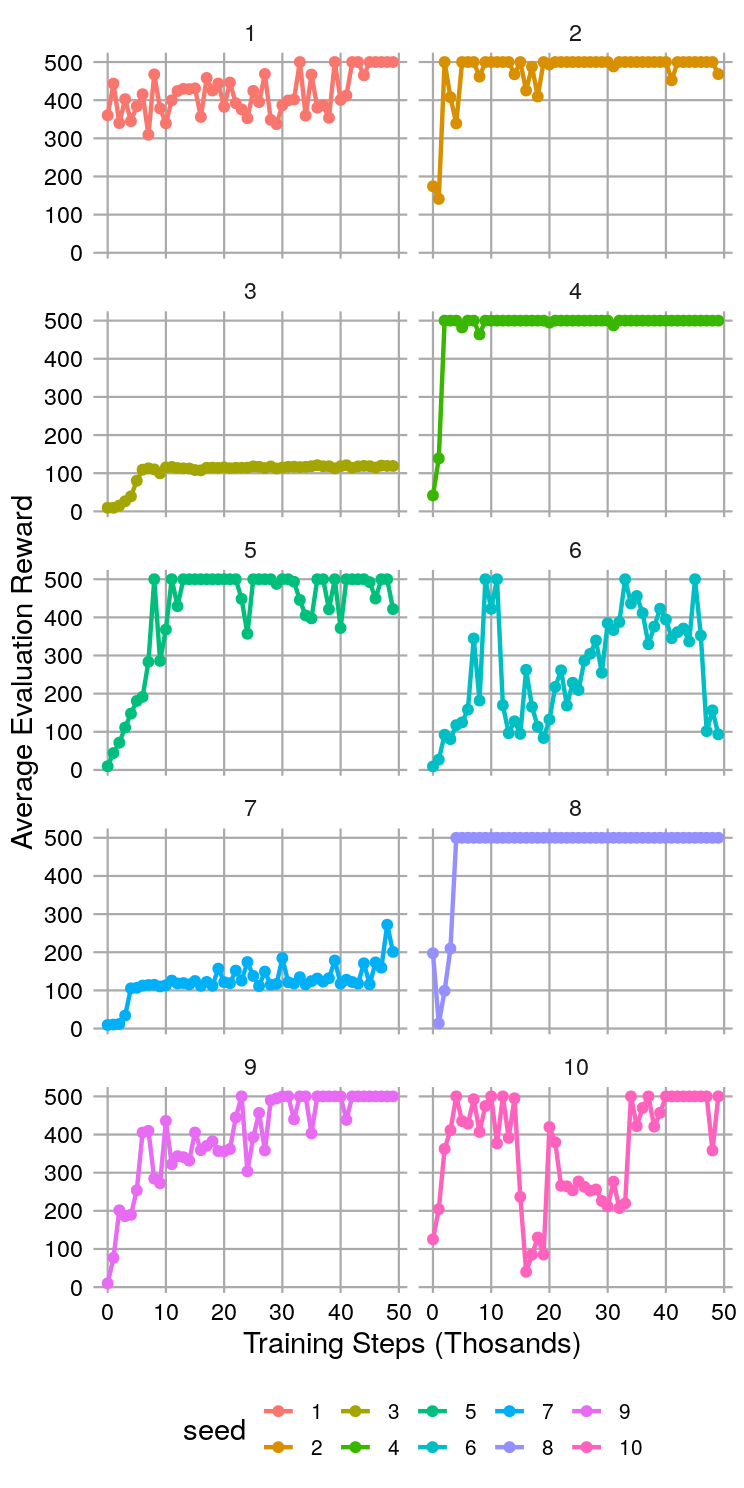
\includegraphics[scale=0.5]{PerDQNCartpole.png}
    }
    \subfloat[BNIG DQN]{
        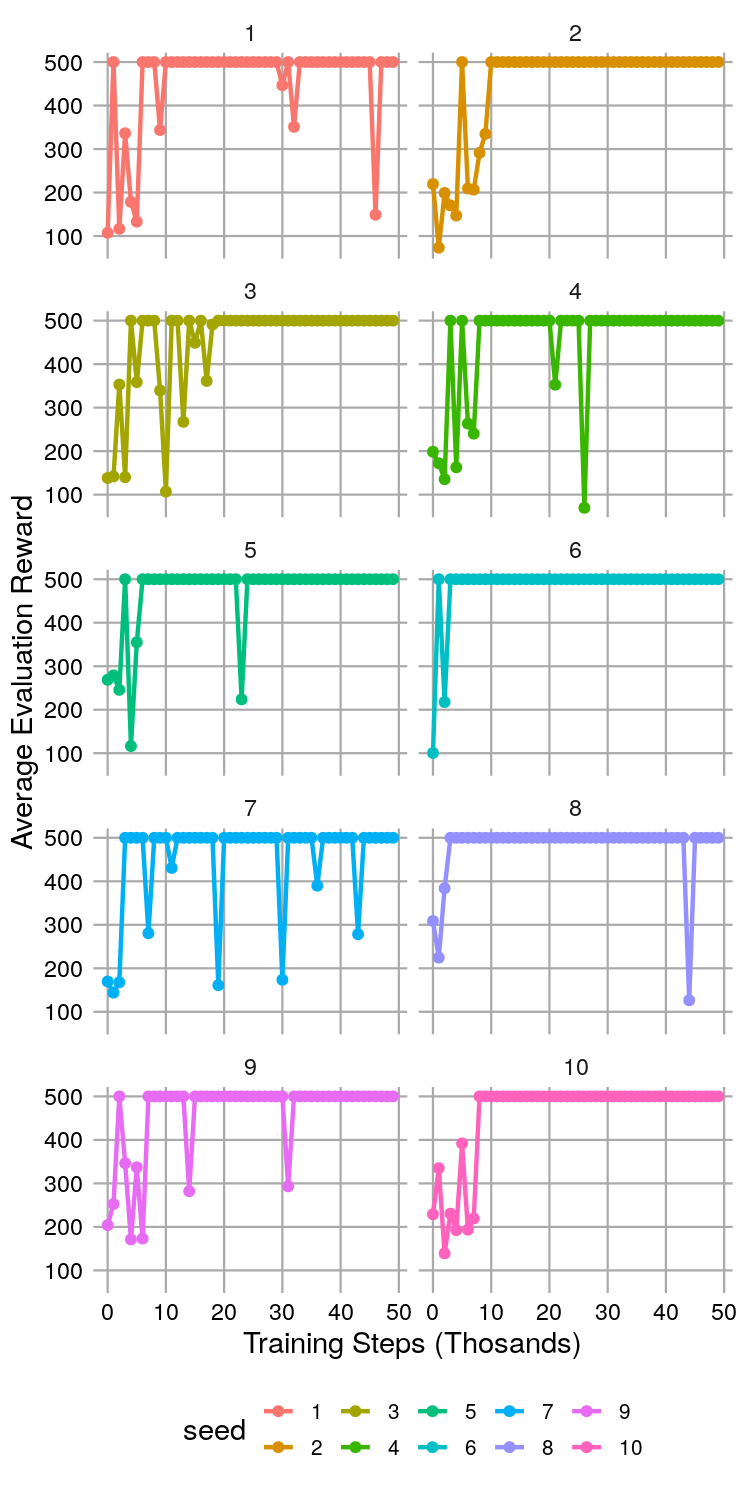
\includegraphics[scale=0.5]{PerBDQNCartpole.png}
    }
    \caption{\textbf{Per Seed DQN and BNIG DQN Performance on Cartpole}: The DQN performance varies a lot from seed to seed. Some seeds the reward is unstable despite seemingly having found a good policy. Other  attempts it never finds an optimal policy. The BNIG DQN always reaches an optimal policy and has more stable results.}
    \label{fig:nn_per_cartpole}
\end{figure}

\begin{figure}[H]
    \centering
    \subfloat[DQN]{
        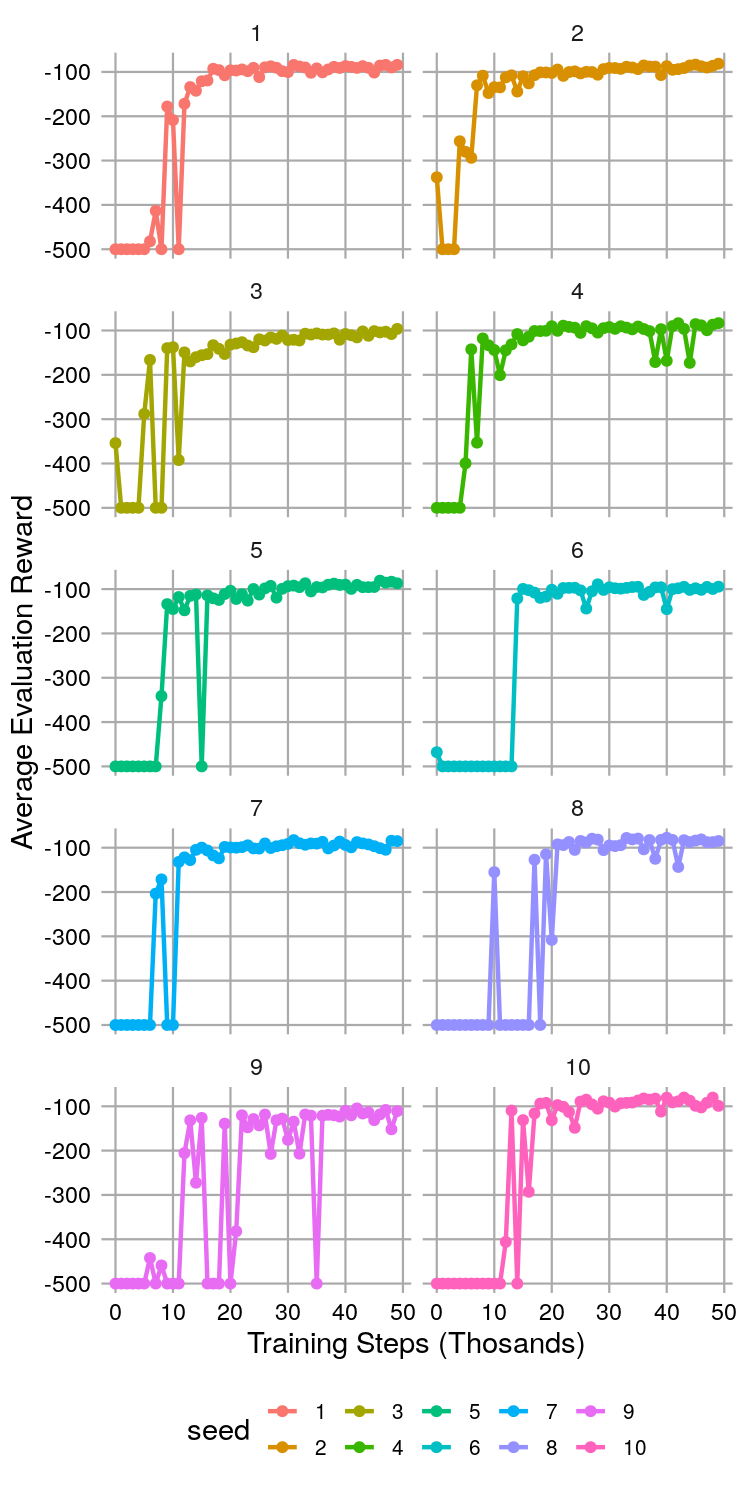
\includegraphics[scale=0.5]{PerDQNAcrobot.png}
    }
    \subfloat[BNIG DQN]{
        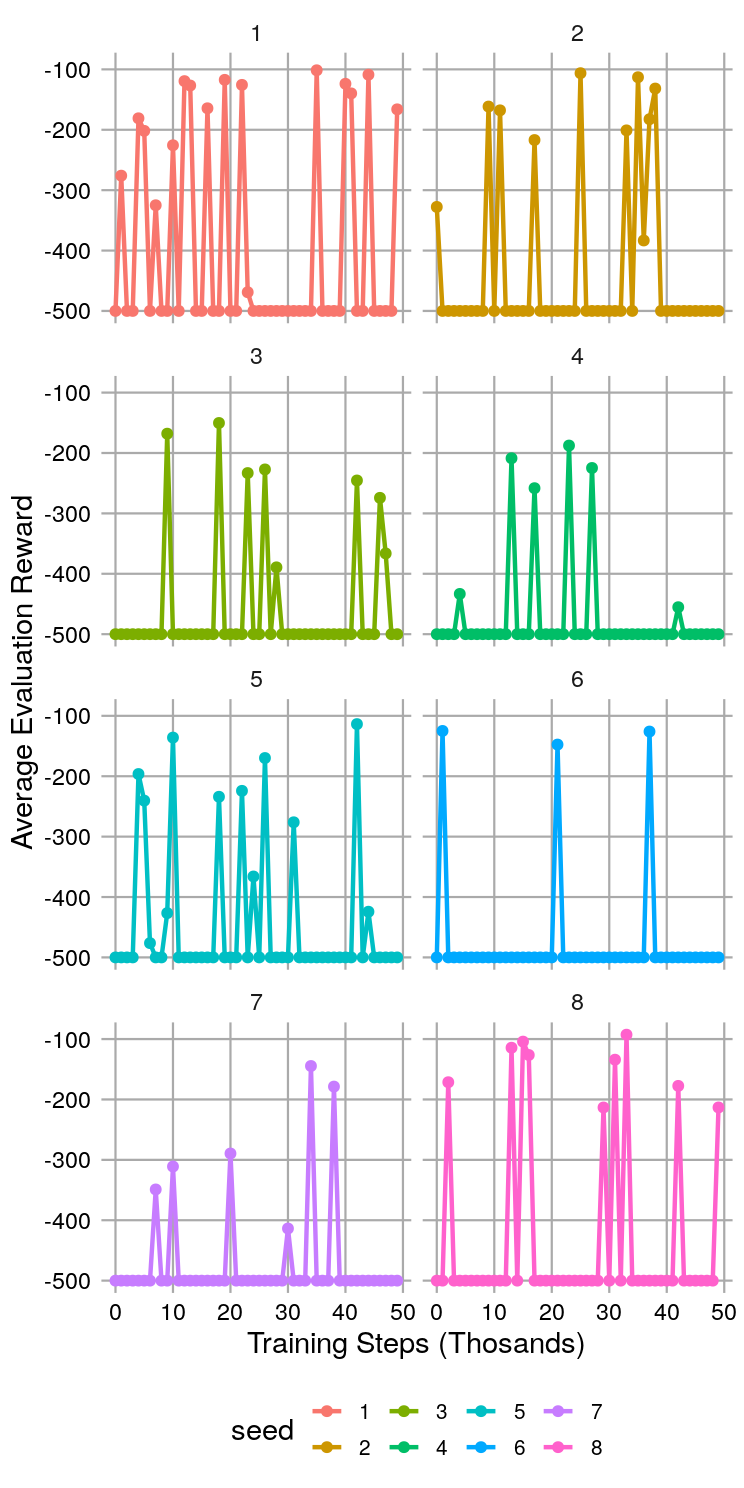
\includegraphics[scale=0.5]{PerBDQNAcrobot.png}
    }
    \caption{\textbf{Per Seed DQN and BNIG DQN Performance on Acrobot}: The BNIG DQN occasionally finds a successful policy but is very unstable. Based on these results the BNIG DQN does not successfully learn the acrobot environment.}
    \label{fig:nn_per_acrobot}
\end{figure}

\section{High Shape BNIG DQN Experiments}


\begin{figure}[H]
    \centering
    \subfloat[DQN]{
        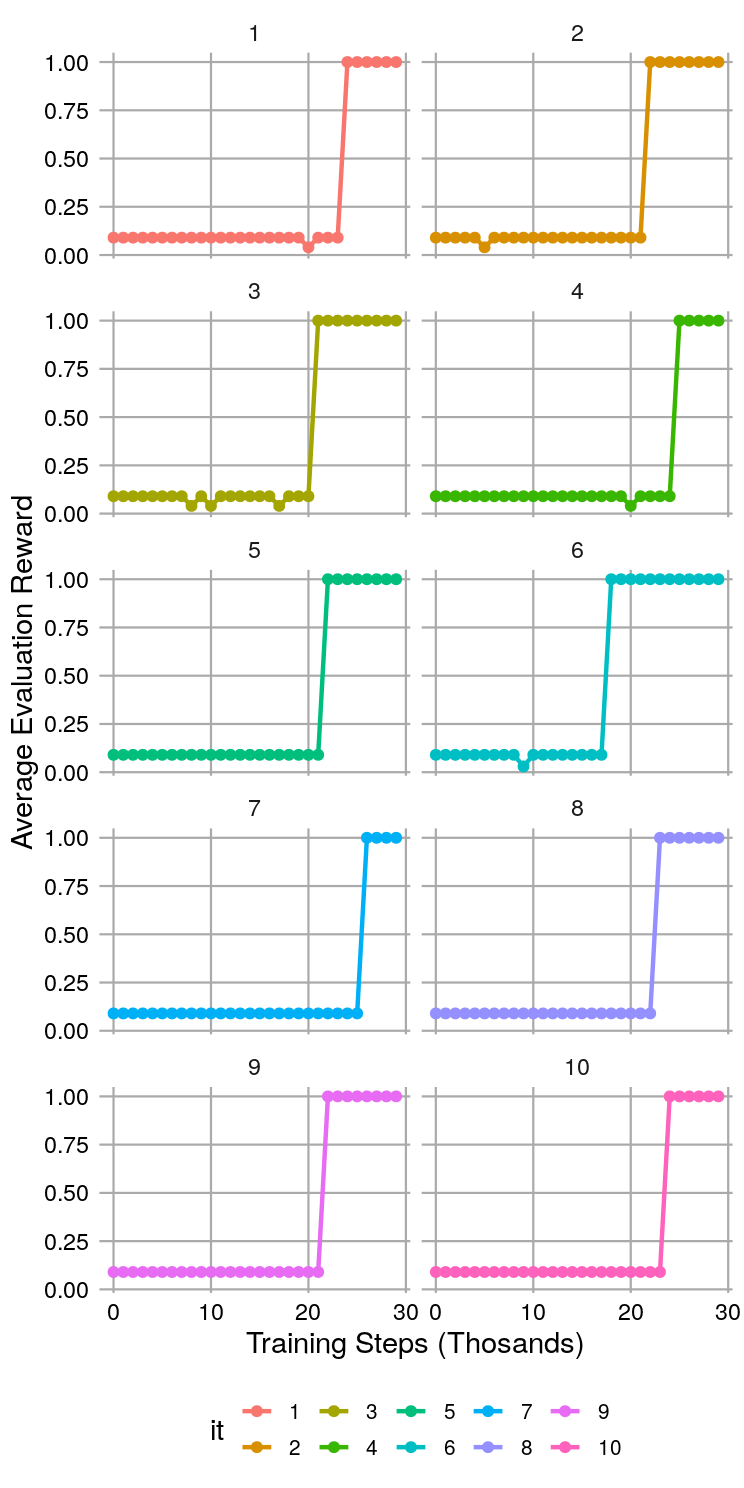
\includegraphics[scale=0.5]{PerDQNCorridor.png}
    }
    \subfloat[High Scale BNIG DQN]{
        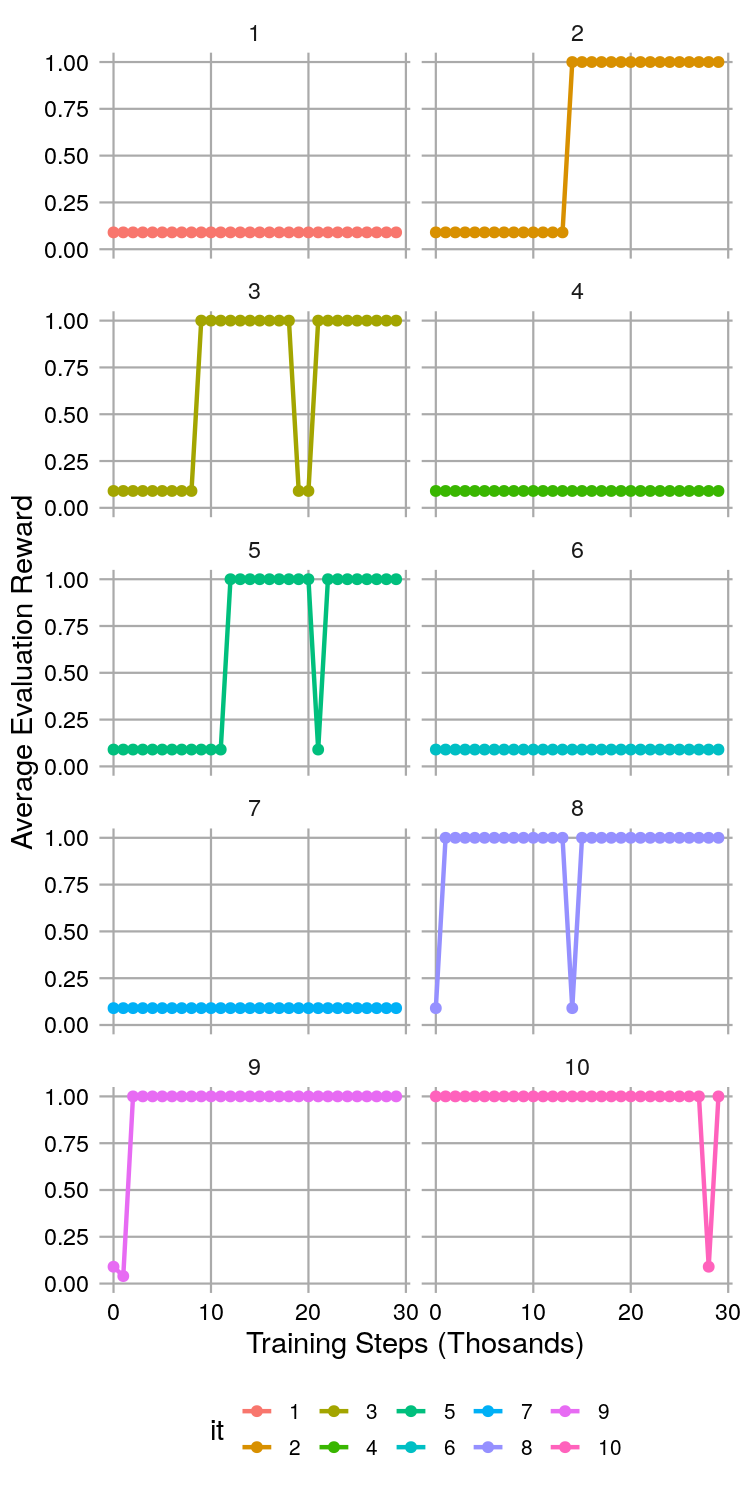
\includegraphics[scale=0.5]{AlphaPerBDQNCorridor.png}
    }
    \caption{\textbf{Per Seed DQN and High Shape BNIG DQN Performance on Corridor}: In 6 of 10 seeds the high shape BNIG DQN successfully learns the corridor environment.}
    \label{fig:alpha_nn_per_corridor}
\end{figure}


\begin{figure}[H]
    \centering
    \subfloat[DQN]{
        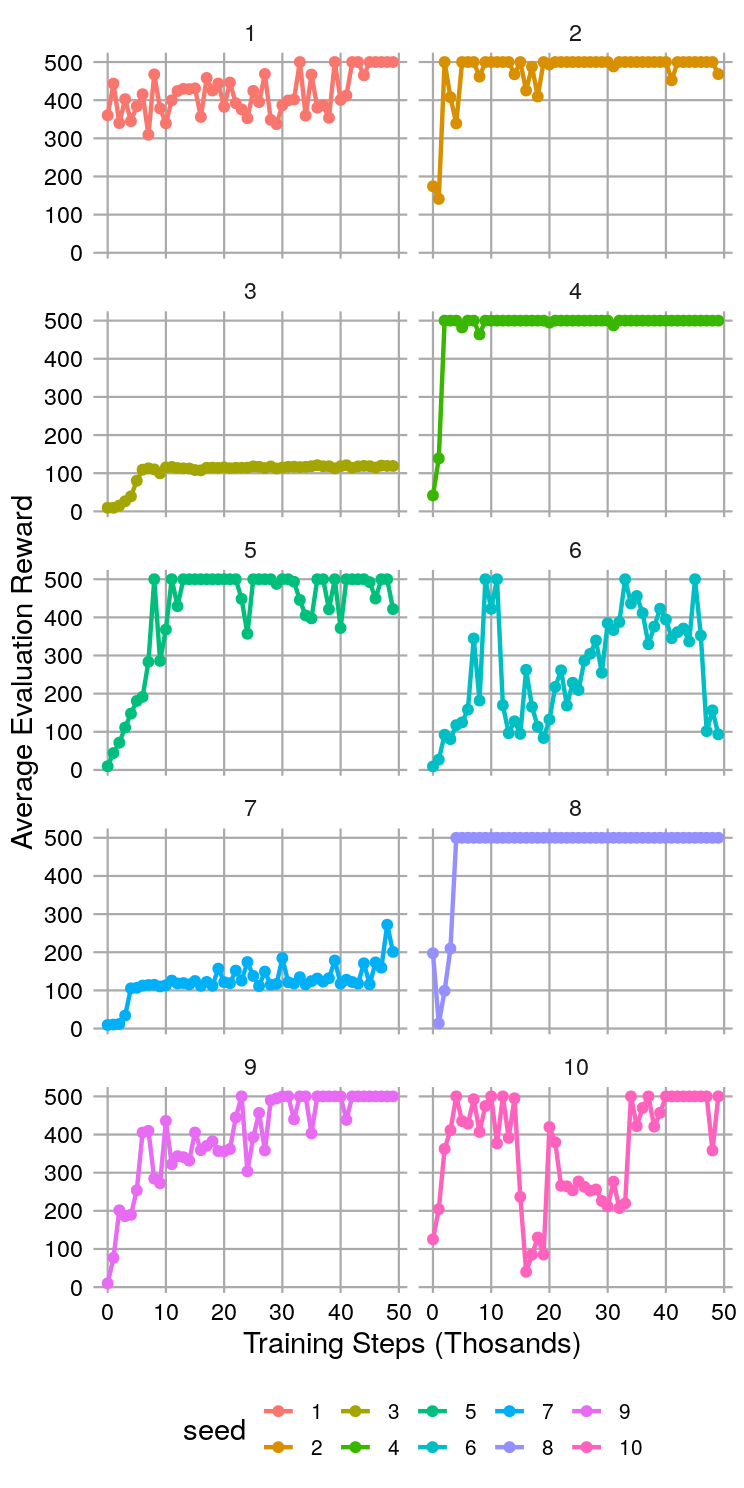
\includegraphics[scale=0.5]{PerDQNCartpole.png}
    }
    \subfloat[High Scale BNIG DQN]{
        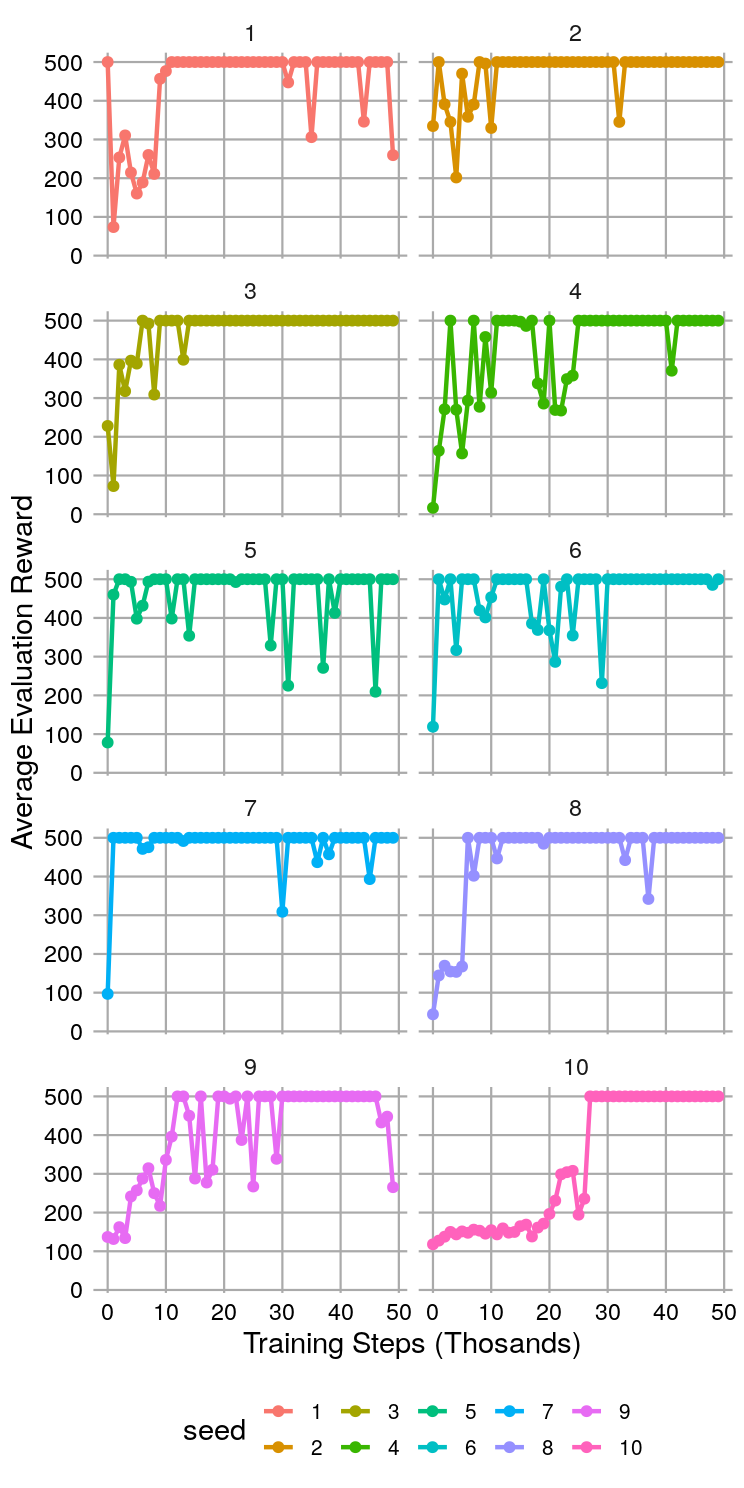
\includegraphics[scale=0.5]{AlphaPerBDQNCartpole.png}
    }
    \caption{\textbf{Per Seed DQN and High Shape BNIG DQN Performance on Cartpole}: The high shape BNIG DQN still outperforms the DQN but has less stable performance than the original BNIG DQN.}
    \label{fig:alpha_nn_per_cartpole}
\end{figure}


\begin{figure}[H]
    \centering
    \subfloat[DQN]{
        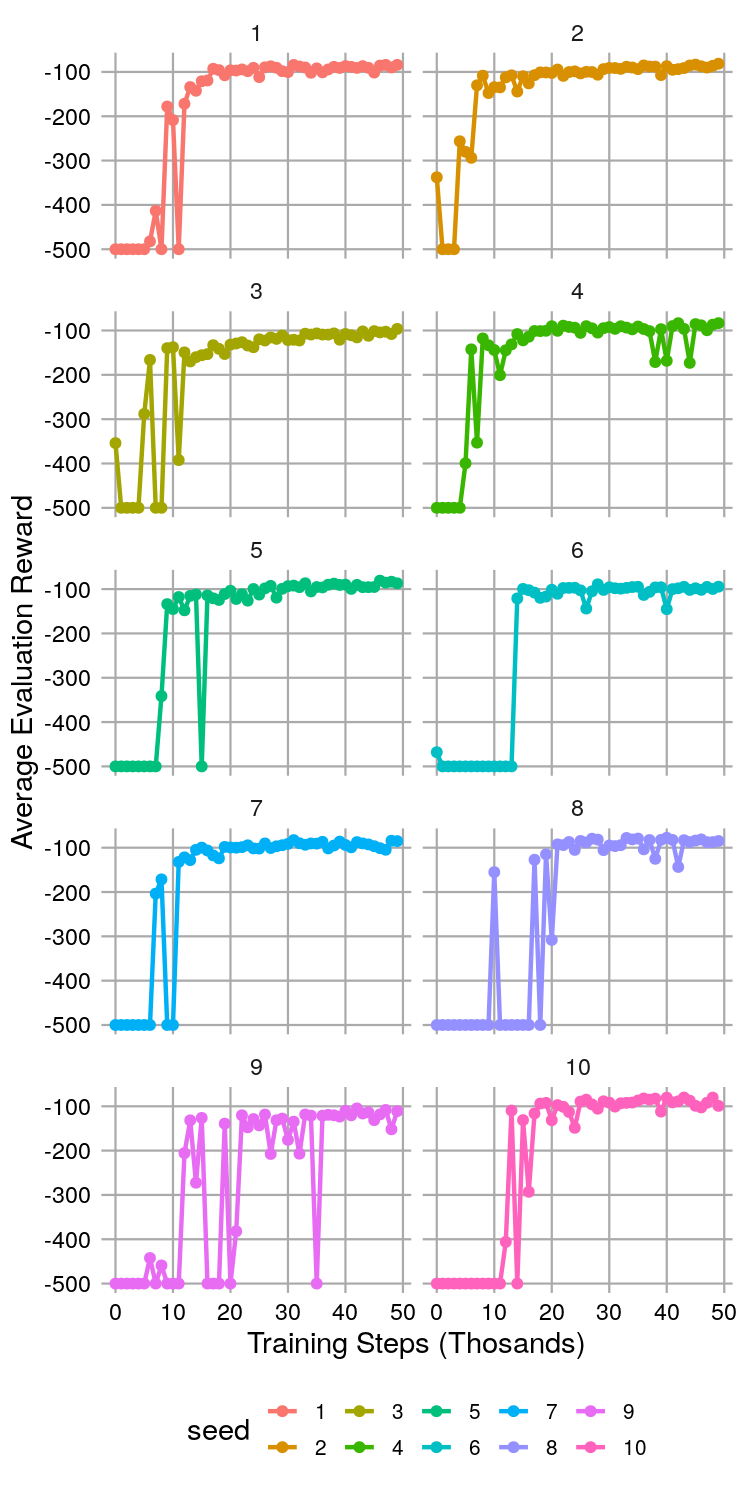
\includegraphics[scale=0.5]{PerDQNAcrobot.png}
    }
    \subfloat[High Scale BNIG DQN]{
        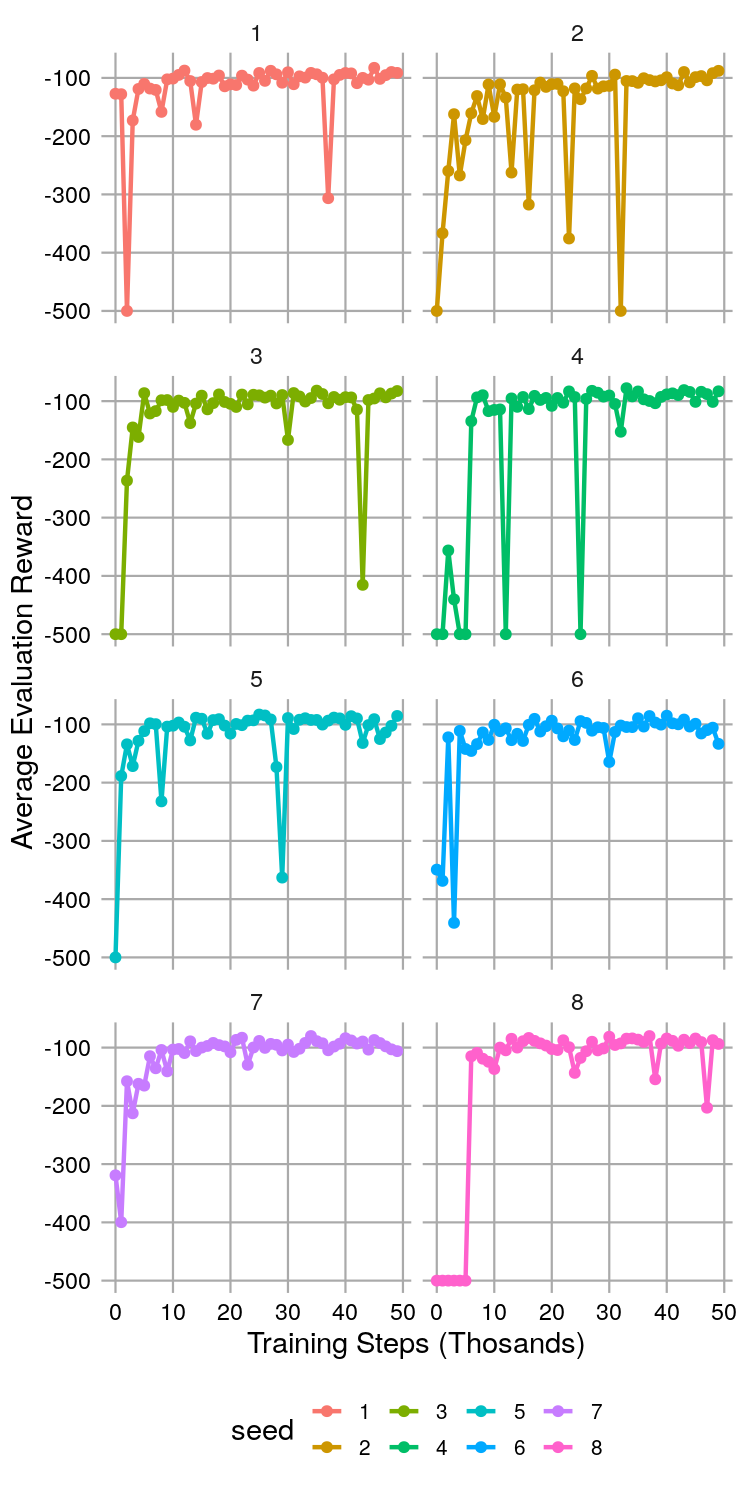
\includegraphics[scale=0.5]{AlphaPerBDQNAcrobot.png}
    }
    \caption{\textbf{Per Seed DQN and High Shape BNIG DQN Performance on Acrobot}: The high shape parameter leads to much better performance on cartpole than the original BNIG DQN. The performance between the DQN and high shape BNIG DQN is similar but the high shape BNIG DQN does learn a successful policy marginally faster.}
    \label{fig:alpha_nn_per_acrobot}
\end{figure}